\documentclass{article}

\usepackage{tikz}
\usetikzlibrary{shapes,arrows}
\begin{document}

\centering
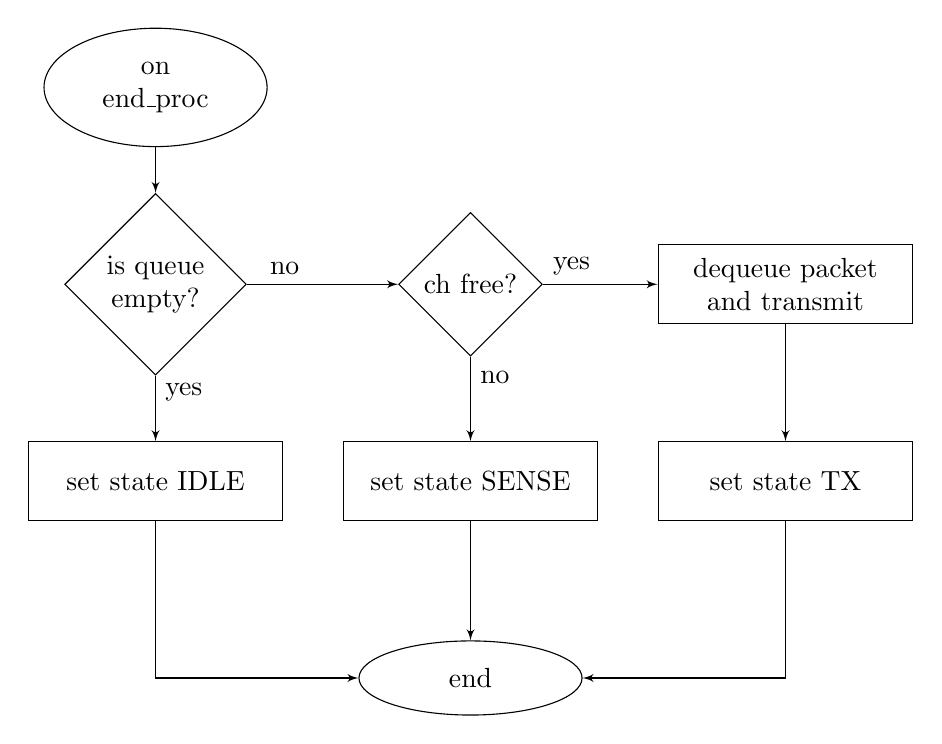
\begin{tikzpicture}[node distance = 2cm, auto]
    \tikzstyle{terminator} = [ellipse, draw,
    text width=4.5em, text centered, inner sep=6pt]
  \tikzstyle{decision} = [diamond, draw,
    text width=4.5em, text centered, node distance=3cm, inner sep=0pt]
  \tikzstyle{block} = [rectangle, draw, text width=3cm, text centered, minimum width=3cm,
    minimum height=1cm]
  \tikzstyle{line} = [draw, -latex']

  % Place nodes
  \node [terminator] (init) {on end\_proc};
  \node [decision, below of=init, node distance=2.5cm] (queue) {is queue empty?};
  \node [decision, right of=queue, node distance=4cm] (count) {ch free?};

    \node [block, right of=count, node distance=4cm] (tx) {dequeue
    packet and transmit};
  \node [block, below of=tx, node distance=2.5cm] (settx) {set state TX};

  \node [block, below of=count, node distance=2.5cm] (setsense) {set
    state SENSE};
  \node [block, below of=queue, node distance=2.5cm] (setidle) {set state IDLE};
  \node [terminator, below of=setsense, node distance=2.5cm] (end) {end};

  % Draw edges
  \path [line] (init) -- (queue);
  \path [line] (queue) -- node [near start] {yes} (setidle);
  \path [line] (queue) -- node [near start] {no} (count);

  \path [line] (count) -- node [near start] {no} (setsense);

  \path [line] (count) -- node [near start] {yes} (tx);
  \path [line] (tx) -- (settx);
  \path [line] (settx) |- (end);

  \path [line] (setsense) -- (end);

  \path [line] (setidle) |- (end);
\end{tikzpicture}


\end{document}
